% shared-layout-id: e74511ba50b8528ae7fbd1e4996e2de36cb501753e1fcc958fda057c20767460
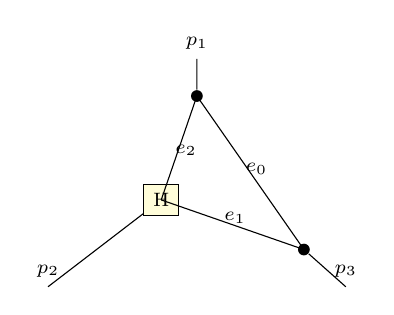
\begin{tikzpicture}[scale=.65,every node/.style={font=\scriptsize}]
\node[circle,fill,inner sep=1.5pt] (v0) at (3.27272727,4.18181818) {};
\node[rectangle,draw,fill=yellow!15] (v1) at (2.57575758,2.15151515) {H};
\node[circle,fill,inner sep=1.5pt] (v2) at (5.36363636,1.18181818) {};
\draw[black] (3.27272727,4.18181818) .. controls (3.96969697,3.18181818) and (4.66666667,2.18181818) .. (5.36363636,1.18181818);
\node at (4.43751246,2.76498802) {$e_{0}$};
\draw[black] (2.57575758,2.15151515) .. controls (3.50505051,1.82828283) and (4.43434343,1.50505051) .. (5.36363636,1.18181818);
\node at (4.01748179,1.80404802) {$e_{1}$};
\draw[black] (3.27272727,4.18181818) .. controls (3.04040404,3.50505051) and (2.80808081,2.82828283) .. (2.57575758,2.15151515);
\node at (3.06181655,3.11943973) {$e_{2}$};
\draw (v0) -- (3.27272727,4.90909091) node[above] {$p_{1}$};
\draw (v1) -- (0.36363636,0.45454545) node[above] {$p_{2}$};
\draw (v2) -- (6.18181818,0.45454545) node[above] {$p_{3}$};
\end{tikzpicture}